\documentclass[tikz,border=3mm,multi=tikzpicture]{standalone}
\usepackage{tikz}
\usetikzlibrary{arrows.meta,positioning}
\begin{document}

% TikZ 1
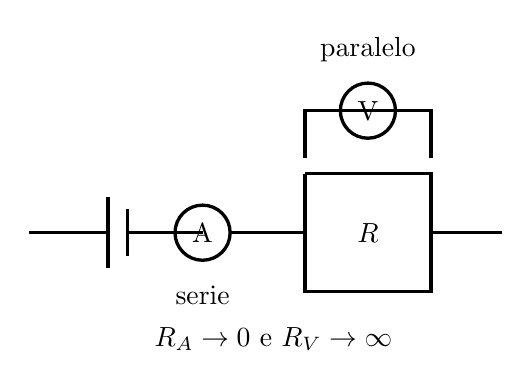
\begin{tikzpicture}[>=Latex]
  \draw[very thick] (0,0) -- (1.0,0);
  \draw[very thick] (1.0,-0.45) -- (1.0,0.45);
  \draw[very thick] (1.25,-0.3) -- (1.25,0.3);
  \draw[very thick] (1.25,0) -- (2.2,0);
  \draw[very thick] (2.2,0) circle (0.35);
  \node at (2.2,0) {A};
  \draw[very thick] (2.55,0) -- (3.5,0);
  \draw[very thick] (3.5,0.75) -- (3.5,-0.75) -- (5.1,-0.75) -- (5.1,0.75) -- (3.5,0.75);
  \node at (4.3,0) {$R$};
  \draw[very thick] (5.1,0) -- (6.0,0);
  \draw[very thick] (3.5,0.95) -- (3.5,1.55) -- (5.1,1.55) -- (5.1,0.95);
  \draw[very thick] (4.3,1.55) circle (0.35);
  \node at (4.3,1.55) {V};
  \node[below] at (2.2,-0.55) {serie};
  \node[above] at (4.3,2.05) {paralelo};
  \node[align=center] at (3.1,-1.35) {$R_A\rightarrow0$ e $R_V\rightarrow\infty$};
\end{tikzpicture}

% TikZ 2
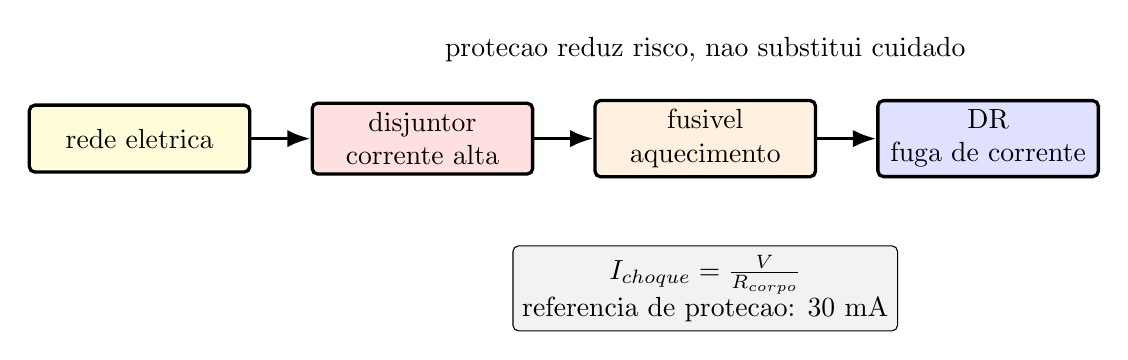
\begin{tikzpicture}[>=Latex,node distance=0.7cm]
  \tikzstyle{box}=[draw,rounded corners=2pt,minimum width=2.8cm,minimum height=0.85cm,align=center,very thick]
  \node[box,fill=yellow!15] (rede) {rede eletrica};
  \node[box,fill=red!12,right=0.75cm of rede] (disj) {disjuntor\\corrente alta};
  \node[box,fill=orange!12,right=0.75cm of disj] (fus) {fusivel\\aquecimento};
  \node[box,fill=blue!12,right=0.75cm of fus] (dr) {DR\\fuga de corrente};
  \draw[very thick,->] (rede) -- (disj);
  \draw[very thick,->] (disj) -- (fus);
  \draw[very thick,->] (fus) -- (dr);
  \node[draw,rounded corners=2pt,fill=gray!10,align=center,below=0.85cm of fus]
    {$I_{choque}=\frac{V}{R_{corpo}}$\\referencia de protecao: $30\ \mathrm{mA}$};
  \node[align=center,above=0.35cm of fus] {protecao reduz risco, nao substitui cuidado};
\end{tikzpicture}

\end{document}
